% =============================================================================
% FILE NAME : 03_concept.tex
% DEPARTMENT: University of Tuebingen
% AUTOR     : Tom Schammo
% =============================================================================
% CONTENT   : Include for chapter "Concept"
% =============================================================================

Goal of this thesis is to implement keyword spotting on the UltraTrail architecture in Rust,
which relies on three components.
A microphone input, Mel Frequency Cepstral Coefficients (MFCC) \cite[Cha 2.5]{rust_pulp} to transform the audio to
a format that UltraTrail can work with and the UltraTrail drivers.\\\\
One PDM and one $I^2S$ microphone have been selected, which exclusively use the $I^2S$ bus and are introduced
in the following section of this chapter.
In order to add support for the UltraTrail architecture and the microphones, the \lstinline{pulissimo_hal}
and \lstinline{pulissimo_pac} crates have to be expanded with drivers and example/test programs.
The PAC contains an SVD file that can be converted to Rust code to provide access to hardware registers
while the HAL crate provides the drivers and example programs for both UltraTrail and the microphones.
Drivers for $I^2S$ and PDM, as well as some example programs have already been implemented,
however neither have been tested nor run before.
Therefore, the implementations need to be tested and potentially modified.


\section{Microphones}

\subsection{Adafruit I2S MEMS Microphone}

\subsubsection{Technical Specification}

The $I^2S$ MEMS microphone from Adafruit \cite{i2s_mic} is a digital microphone.
It requires a supply voltage between \SI{1.62}{\volt} and \SI{3.6}{\volt} while drawing a current of \SI{600}{\micro\ampere}.
During sleep mode the current draw is reduced to \SI{10}{\micro\ampere}, and the clock frequency is lowered from anything between
\SI{2048}{\kilo\hertz} and \SI{4096}{\kilo\hertz} to \SI{900}{\kilo\hertz}.
A logical high is read for any voltage between 65\% of the supply voltage ($V_{DD}$) and $V_{DD}$ + \SI{0.3}{\volt},
and a logical low is read for any voltage between \SI{-0.3}{\volt} and 35\% of $V_{DD}$ \cite{i2s_mic_datasheet}.

\subsubsection{Pinout}

The breakout board has 6 pins, $V_{DD}$ and Ground (GND), which are responsible for power, as well as 4 data pins.
The output of the microphone can be read on 'Data Out' (DOUT), the channel (right/left mono audio) can be changed by
changing the voltage of the 'Select' (SEL) pin, which is set to low (left) by default.
The 'bit clock' (BCLK) is the main clock of the device that determines when data is transmitted, and the 'left/right clock' (LRCLK)
controls whether data is transmitted on the left or right channel.
The LRCLK will also be referred to as 'Word Select' (WS) in some instances \cite{i2s_mic_pinout}.

\subsubsection{Timing}

Figure~\ref{fig:i2s_timing} shows the timing diagram of the $I^2S$ microphone.
A clock period should take between \SI{244.14}{\nano\second} and \SI{488.28}{\nano\second}.
A high or low pulse on the clock should be 35\% of the duration of a period.
The maximum delay of the data from a rising edge of the clock should be \SI{65.92}{\nano\second}
and the clock should take no longer than \SI{3.75}{\nano\second} to rise from low to high \cite{i2s_mic_datasheet}.
\\
WS has to change on a falling edge of the clock (BCLK in this case).
Data is sent with the MSB first and delayed by one clock cycle after a change in WS.

\begin{figure}[htb]
    \centering
    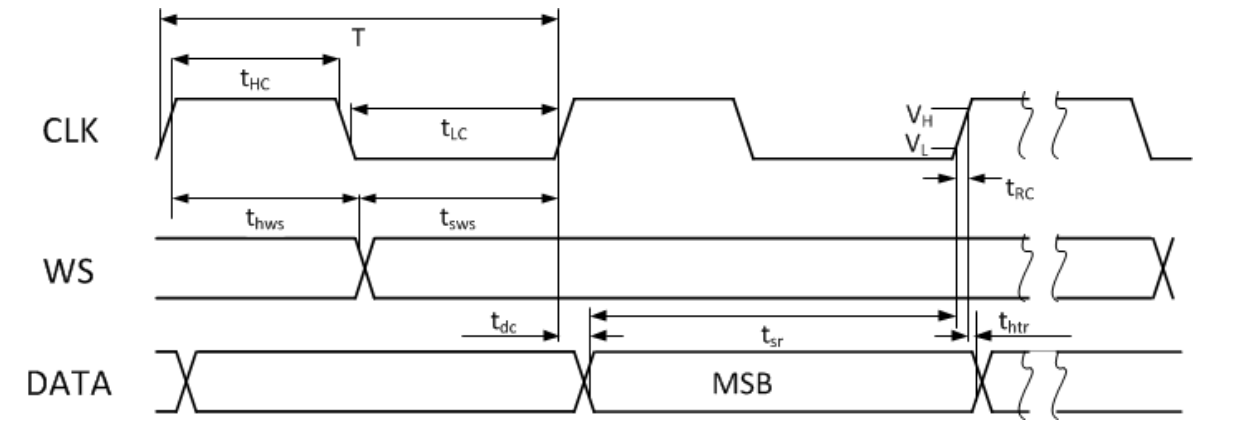
\includegraphics[width=0.9\textwidth]{figures/i2s_timing.png}
    \caption[Timing diagram of the SPH0645LM4H-B $I^2S$ mic \cite{i2s_mic_datasheet}]{Timing diagram of the $I^2S$ microphone}
    \label{fig:i2s_timing}
\end{figure}

\subsection{Adafruit PDM MEMS Microphone}

\subsubsection{Technical Specification}

The PDM MEMS microphone from Adafruit \cite{pdm_mic} is a digital microphone.
It uses the $I^2S$ bus to communicate, but instead of the typical 24 bit encoding of $I^2S$ microphones, PDM microphones only use 1 bit.
It requires a supply voltage between \SI{1.64}{\volt} and \SI{3.6}{\volt} while drawing a current of \SI{600}{\micro\ampere}, with a clock
frequency from \SI{1}{\mega\hertz} to \SI{3.25}{\mega\hertz}.
However the clock frequency should be reduced to a maximum of \SI{0.23}{\mega\hertz} while the microphone is in 'power-down' mode.
During power down mode the current draw is reduced to \SI{20}{\micro\ampere}.
A logical high is read for any voltage between 65\% of ($V_{DD}$) and $V_{DD}$ + \SI{0.3}{\volt},
and a logical low is read for any voltage between \SI{-0.3}{\volt} and 35\% of $V_{DD}$ \cite{pdm_mic_datasheet}.

\subsubsection{Pinout}

The breakout board of the PDM microphone, in contrast to the breakout board of the $I^2S$ microphone, only has 5 pins.
$V_{DD}$ and Ground (GND), serve the same purpose, but it only needs 3 data pins.
The output of the PDM microphone can be read on 'PDM Data Out' (DAT), and the PDM microphone also has a SEL pin (also referred to as L/R in the timing diagram),
which works the same way as it does in the $I^2S$ microphone.
However, it only has one clock line (CLK), and no WS \cite{pdm_mic_pinout}.

\subsubsection{Timing}

Figure~\ref{fig:pdm_timing} shows the timing diagram for the PDM microphone.
Based on the clock frequency, a period in normal mode should take between \SI{308}{\nano\second} and \SI{1000}{\nano\second}.
The right channel (PDM R) is latched onto the rising edge of the clock and is enabled if the L/R pin is set accordingly.
It is disabled on the falling edge of the clock.
The left channel (PDM L) is latched onto and thus enabled on a falling edge of the clock (assuming L/R is set accordingly),
and disabled on a rising edge.
According to data acquired from design simulations by manufacturer,
PDM L and PDM R takes at least \SI{18}{\nano\second}, while disabling PDM L and PDM R takes at most \SI{16}{\nano\second}.


\begin{figure}[htb]
    \centering
    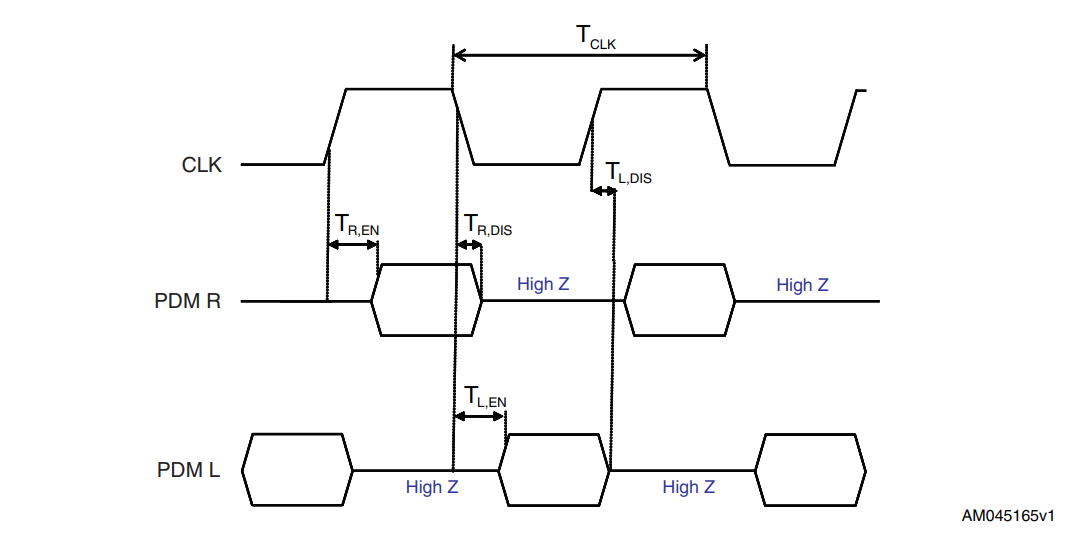
\includegraphics[width=0.9\textwidth]{figures/pdm_timing.png}
    \caption[Timing diagram of the MP34DT01-M PDM MEMS mic \cite{pdm_mic_datasheet}]{Timing diagram of the PDM MEMS microphone}
    \label{fig:pdm_timing}
\end{figure}

\section{Experiments}

\subsection{Microphones}

A variety of tests are used to determine the functionality of the microphones.
The first test simply consists of playing some sort of noise and analyzing the output of the microphones to see if
they respond in some predictable manner.
After that finer testing is carried out by playing a sound that represents a perfect sign wave,
which should yield a perfect sign wave on the end of the microphones as well.\\
An array of equipment is used to analyze the output of the microphones; namely a logic analyzer, an oscilloscope
(for debugging purposes), as well as a few python tools to save and analyze the output data.

\subsection{UltraTrail}

The UltraTrail test makes sure that configuration changes have the desired effect (bits are correctly set in the correct registers),
and the AI accelerator is tested using a predefined set of input data.
After the input data is loaded correctly, the accelerator is started and will trigger a hardware-peripheral event when it is done.
After that the results are compared with the desired results, which finally determines the functionality of the drivers.
